\documentclass[../main.tex]{subfiles}
\graphicspath{{\subfix{../images/}}}
\begin{document}

  Para o desenvolvimento do projeto, foi criada uma metodologia própria a ser seguida, composta por quatro fases sequenciais, conforme ilustrado na figura \ref{fig:metodologia} e detalhado a seguir. \textbf{\textcolor{red}{Colocar como apêndice?}}

  \begin{figure*}[h]
    \centering
    \caption{Metodologia}
    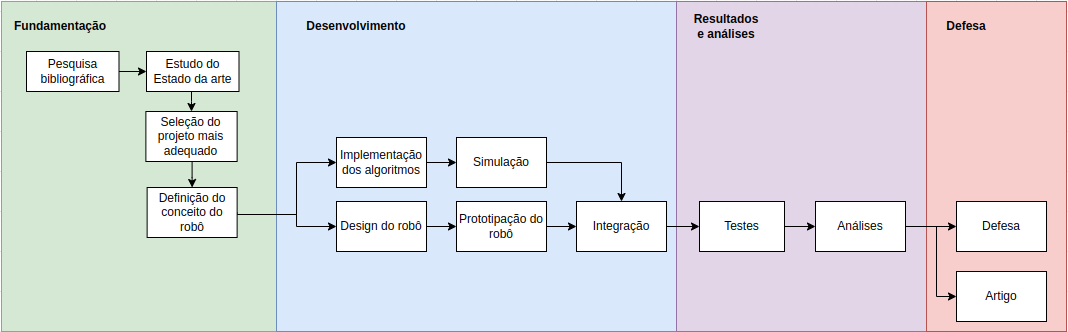
\includegraphics[width=\textwidth]{metodologia.png}

    Fonte: Proprio autor
    \label{fig:metodologia}
  \end{figure*}

  \subsection{Fundamentação}
  A primeira fase da metodologia tem como objetivo buscar referências que possam embasar o estudo e servir de padrão para o design e desenvolvimento do projeto.

  Durante essa fase de Fundamentação, o primeiro a ser feito são pesquisas bibliográficas, com o intuito de selecionar artigos úteis e correlatos ao projeto. \textcolor{red}{Para isso, foi utilizado o \textit{Método Bili}.}

  A partir dessas pesquisas, é possível realizar um Estudo do Estado da Arte, selecionando, a partir de um \textcolor{red}{Benchmarking} realizado com robôs quadrúpedes, projetos que possam servir de referência para o desenvolvimento, definindo os \textcolor{red}{conceitos, funcionalidades e design} que o projeto deverá ter.

  \subsection{Desenvolvimento}
  Durante esta etapa da metodologia, ocorre o desenvolvimento do robô propriamente dito. Inicialmente, duas etapas ocorrem de forma parelela, sendo elas a implementação e simulação dos algoritmos (em ambiente computacional) e a definição e prototipação do design do robô.

  Durante a implementação de algoritmos e simulação, são inicialmente elaborados o diagrama de blocos do sistema e a arquitetura de software do controlador, de forma a padronizar e documentar o desenvolvimento do projeto. A partir disso, os algoritmos de cinemática e controle podem ser implementados e testados em simulação. Para auxiliar e possibilitar o desenvolvimento do projeto, algumas ferramentas e \textit{Softwares} serão utilizados. O ROS - Robot Operating System é um conjunto de bibliotecas e ferramentas de \textit{software Open Source} que auxiliam no desenvolvimento de aplicações robóticas. O ROS Humble, nativo para Ubuntu 22.04, será utilizado, por possuir boa documentação e comunidade ativa, além de possuir pacotes muito úteis para o desenvolvimento do robô. 

  Em paralelo com o desenvolvimento de software, a prototipação e construção do robô é realizada, através da elaboração dos desenhos mecânicos e projetos eletro-eletrônicos. Esta etapa inclui também a impressão 3D das partes mecânicas projetadas, teste dos atuadores e sensores e configuração e comunicação entre o processador e os servo-motores Dynamixel \textcolor{red}{modelo?} que serão utilizados, culminando na montagem física do protótipo funcional. Os Softwares OnShape e XXXX serão utilizados para o desenvolvimento do CAD do robô e para seu projeto elétrico, respectivamente.

  Após essas etapas, é possível realizar a integração dos algoritmos no protótipo físico, de forma a validar o desenvolvimento realizado em ambiente computacional em um robô no mundo real.

  \subsection{Resultados e Análises}
  Durante a etapa de resultados e análises, além das inferências visuais, a performance do robô no mundo real foi analisada por meio de alguns testes. Neste momento procuramos avaliar de forma estatística se os algoritmos implementados possuem a resposta esperada e se o protótipo atende aos requisistos funcionais do projeto, ou seja, é capaz de andar por terreno regular e irregular, superar obstáculos  de 200 mm e de suportar uma carga de até 2 Kg.

  O primeiro experimento consiste em observar a capacidade do protótipo em mover o pé por uma dada trajetória cicloidal, calculada pelo planejador de trajetória. Para isso, o corpo do robô está estático e suspenso por um suporte, logo, não há carga significativa sobre os motores. As trajetórias foram calculadas considerando a altura de passo de 0,05 m, período de 0,5 segundos e uma resolução de 25 pontos distribuídos de forma homogênea.
  
  Durante o segundo teste foi analisado se o robô atende à uma velocidade solicitada e observado a estabilidade do corpo, considerando dois tipos de terreno, um plano e outro irregular. Este experimento consiste em enviar um comando de velocidade linear, para frente, e medir o tempo que o robô levou para alcançar 1,5 m, dessa forma, obtêm-se a velocidade média do robô.  Além disso, a fim de avaliar a contribuição do controle de rotação do robô, parte dos experimentos foi realizado com esta funcionalidade e outra sem. A estabilidade do robô foi mensurada por meio dos dados de orientação fornecidos pelo IMU e o passo utilizado possui as especificações citadas no primeiro experimento. Dessa forma, os testes foram organizados em quatro combinações, variando a composição do terreno, concreto ou pequenas pedras, e o uso ou não do controle de rotação.
  
  No terceiro experimento foi avaliado se o Caramelo é capaz de andar por terrenos inclinados. Então, foi contruída uma rampa com uma inclinação de 5,336\degree, pela qual o robô deveria subir e descer de forma teleoperada. Por fim, para o quarto teste foi proposto que o Caramelo atravessasse degraus de alturas diferentes, também de forma teleoperada, a fim de encontrar a máxima altura de obstáculo que o robô consegue superar.

  \subsection{Defesa}
  Esta é a última etapa da metodologia, que consiste na finalização e revisão do artigo e na apresentação de defesa do trabalho perante a banca avaliadora. 

\end{document}
